\chapter{生成式人工智慧} \label{chap:generative_ai}

\section{不訓練模型的情況下強化語言模型的方法} 
\subsection{拆解問題}
把複雜的任務拆解為簡單的子任務,並讓AI分別解決各個步驟。\autoref{fig:CoT}是叫模型思考(Chain of Though, CoT)解決數學問題的流程圖。
\begin{figure}[htbp]
    \centering
    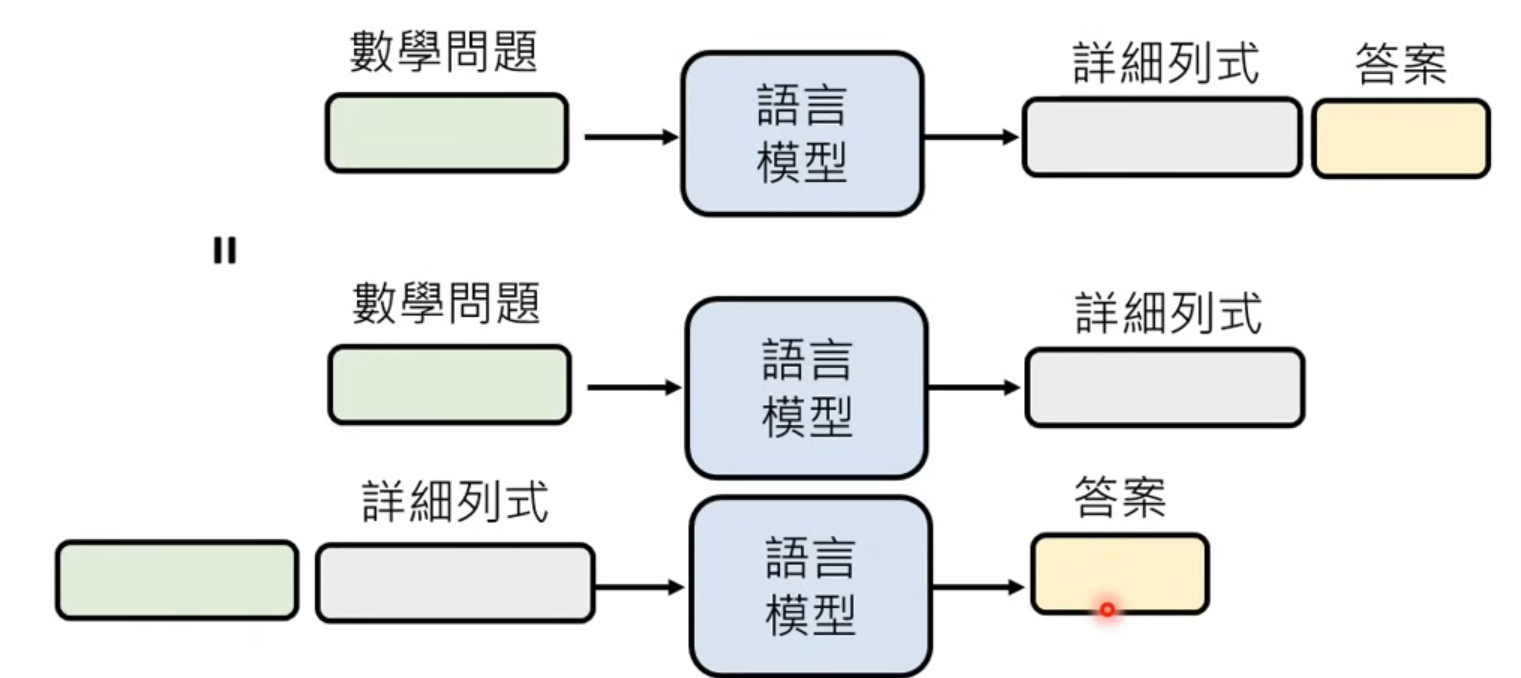
\includegraphics[width=0.7\linewidth]{images/w13/CoT.png}
    \caption{Chain of Thought流程}
    \label{fig:CoT}
\end{figure}
\subsection{檢查自己的錯誤}
語言模型再做文字接龍的時候,有時會產生一些不存在的東西,這時可以讓他檢查自己提供的答案是否正確。
但是在這個過程中\textbf{語言模型沒有被訓練},模型的函式是固定的。
\begin{figure}[htbp]
    \centering
    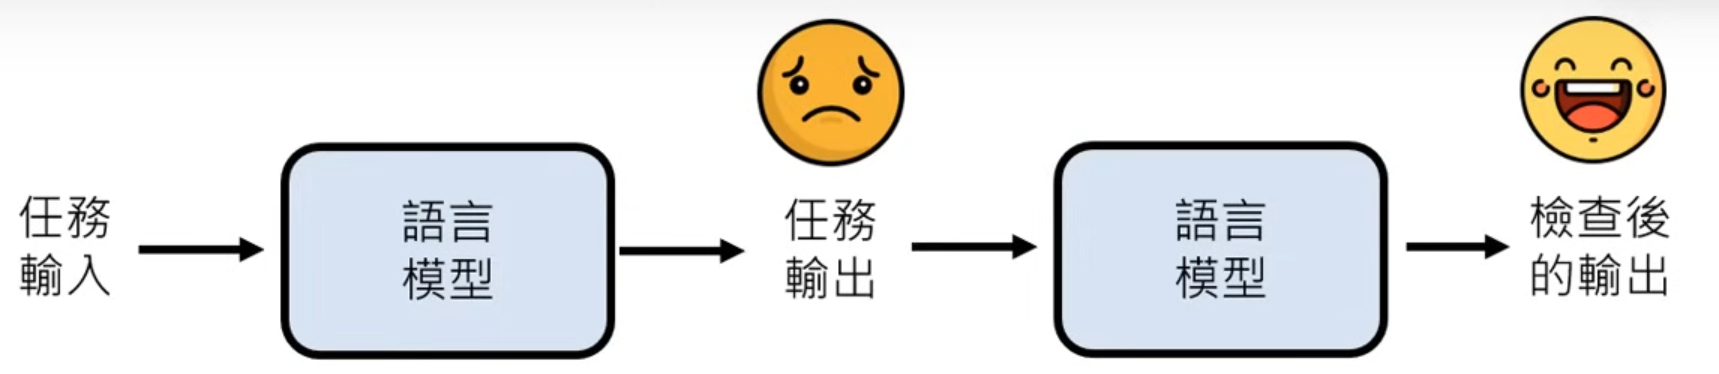
\includegraphics[width=0.7\linewidth]{images/w13/mistake.png}
    \caption{檢查錯誤}
    \label{fig:w13-mistake}
\end{figure}
\subsection{Retrieval Augmented Generation}
有一些困難問題語言模型很難依靠文字接龍解決,這時可以搭配搜尋引擎從網路或資料庫得到結果(額外資訊),再將問題與額外資訊結合給語言模型去做生成提高正確率。
\begin{figure}
    \centering
    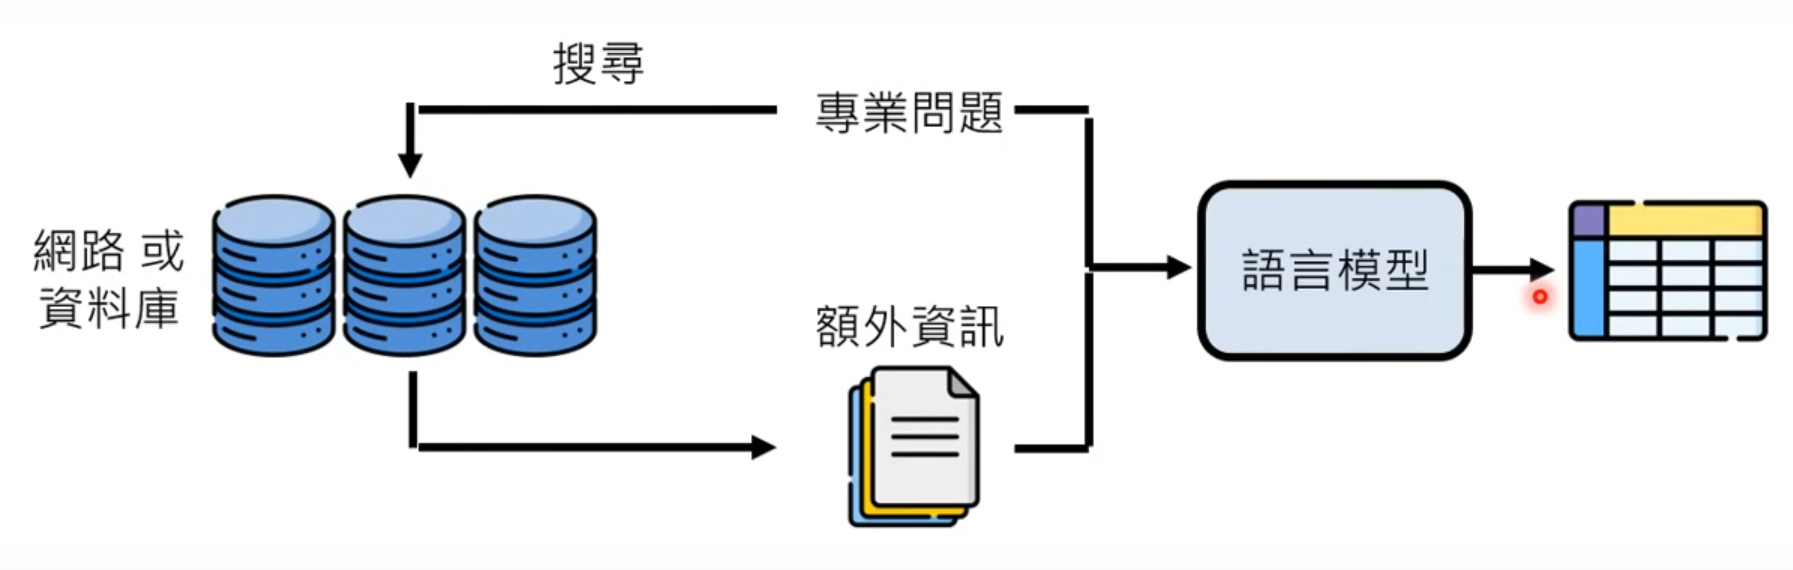
\includegraphics[width=0.7\linewidth]{images/w13/RAG.png}
    \caption{Retrieval Augmented Generation}
    \label{fig:w13-RAG}
\end{figure}
